\newpage	
\section{Reconocimiento de texto en escenas naturales}

	En el capítulo anterior, se desarrollaron los conceptos necesarios para entender las bases del aprendizaje supervisado y los clasificadores probabilísticos. Todos estos conceptos sirven para entender los principios sobre los que se asienta el trabajo realizado por Wang et. al. en \cite{wang}. El trabajo de los autores, abarca el reconocimiento de texto en escenas naturales en todas sus etapas. En particular, una de ellas es el reconocimiento de caracteres.
	
	En este capitulo se van a presentar dos implementaciones: la provista originalmente por Wang et al. en \cite{wang} y la realizada en este trabajo basándose en la primera. Solamente se van a desarrollar los temas referentes al reconocimiento de caracteres ya que el presente trabajo se enfoca únicamente en ese problema. Como complemento a ambas implementaciones, hay una sección dedicada al papel que juegan las imágenes en ambos trabajos. Se explica la importancia de las mismas y qué método se utiliza para la extracción de las características.
	
	
	\subsection{Introducción}

	En el trabajo que realizaron Wang et al., los autores identificador el problema que había al detectar y reconocer palabras en imágenes naturales. Ellos identifican, que si bien las actuales aplicaciones de OCR se manejan bien con documentos escaneados, el texto adquirido en entornos naturales (también referido como texto de escena) se ha vuelto más frecuente. Todo esto debido al aumento de dispositvos que son capaces de extraer dicha información, sean estos celulares, tabletas o cámaras.
	
	Con la salida del primer dataset público denominado \textit{ICDAR}, el cual resaltaba el problema de detectar y reconocer texto de escena, los organizadores del mismo, identificaron cuatro subproblemas.
	\begin{itemize}
		\item La clasificación de caracteres recortados.
		\item Detección de texto en la imagen completa.
		\item El reconocimiento de palabras recortadas.
		\item El reconocimiento de palabras en la imagen completa.
	\end{itemize}
	
	Dada esta problemática, los autores se enfocaron en el problema del reconocimiento de texto. Para poder encarar esto, incorporaron una lista de palabras (i.e., un lexicón) para detectar y leer.
		
	Para esto, ellos construyen y evaluan dos sistemas. El primero consiste en un pipeline de dos etapas que consiste en la detección de texto seguido del reconocimiento a partir de un destacado motor de OCR. El segundo, es un sistema arraigado en el reconocimiento de objetos genéricos, el cual es una extensión de un trabajo que realizaron anteriormente \cite{WB10}.
	
	Sus contribuciones son las siguiente:
		\begin{itemize}
			\item Evaluan la performance en la detección y el reconocimiento de palabras de un enfoque de dos etapas que consiste en un detector de texto (que es estado del arte) y un destacado motor de OCR.
			\item Construyen un sistema basado en su trabajo anterior \cite{WB10} y muestran que sus pipelines de reconocimiento realizan una mejor tarea a comparación al pipeline convencional de OCR.
		\end{itemize}	
	
	\newpage
\subsection{Clasificación de imágenes naturales}

	Para poder comprender de mejor manera la sección \ref{subsection: wang_recon_caracteres}, es necesario adentrarse en las particularidades que caracterízan a las imágenes naturales. Dado que, como se ha detallado anteriormente, no es sencillo trabajar con este tipo de imágenes, la siguiente sub-sección se enfoca en las características de las escenas naturales. Las siguientes sub-secciones van a explicar conceptos como el de gradiente que es necesario para poder entender a los descriptores HOG (ver \ref{subsection:hog}) usados tanto por Wang et. al. en \cite{wang}, como por el presente trabajo. Finalmente, se explica el proceso de binarización, necesario para poder usar el clasificador \textit{Random Ferns}.

	\subsubsection{Características}

Las características en las imágenes naturales son muy variadas. Dentro de las mismas podemos encontrar las variaciones de intensidad en la iluminación, la resolución, el ángulo en el que son tomadas, el fondo, las texturas, entre otros. Mas específicamente, dependiendo del objeto que se esté analizando, por ejemplo, texto, surgen más características como el tipo de fuente, el tamaño, la posición y orientación de los caracteres, la contaminación que pueda llegar a tener el texto por suciedad u oclusión, etc. La infita variedad que es posible encontrar en este tipo de imágenes, dificultan el trabajo de reconocimiento sobre ellas por lo que, en general, es necesario realizar un pre-procesamiento antes de usarlas.

	En el caso del reconocimiento de texto, dada la gran cantidad de formas en que se puede encontrar la imagen de un carácter, es necesario encontrar algún método que extraiga las características mas representativas para poder distinguilo. Para poder analizar los caracteres en las imágenes naturales, uno de los enfoques que adoptan Wang et al. en \cite{wang} es el de trabajar con el descriptor HOG de cada imagen. Para poder entender que es un descriptor HOG (que se detalla en \ref{subsection:hog}), primero es necesario comprender el concepto de gradiente que se explica a continuación.
	
	%	Desde la aparición de las primeras fotografías, las personas han buscado ``inmortalizar'' escenas, objetos o personas, con el objetivo de, en el area de la ciencias, extraer información útil de las mismas que pueda ser utilizada para su analisis o estudio. Con el surgimiento de los primeros formatos digitales, la necesidad pasó por encontrar métodos automáticos que permitieran clasificar y reconocer elementos dentro de las imágenes. Desde reconocer texto manuscrito, texto en carteles publicitarios, patentes, personas, animales hasta identificar zonas con agua en una imagen satelital. La cantidad de potenciales aplicaciones que se pueden obtener es enorme. Es por eso que en campos de investigación como visión por computadora, este es un tema de interés. Sin embargo, la clasificación en imágenes naturales no es una tarea para nada sencilla. Por ejemplo, en el reconocimiento de texto, las imágenes naturales contienen muchas información ``extra'' que se tiene que tener en cuenta. Ya sea la existencia de otros objetos ajenos a la clasificación, es decir, elementos que no son texto como así también variaciones propias en las características de la misma imagen (se detallan más adelante en esta sección).
	
	Hoy en día se ha avanzado mucho en el área de la clasificación en escenas naturales. Se han desarrollado muchas aplicaciones como aquellas capaces de reconocer personas \cite{DT05}, hasta las que pueden identificar patentes \cite{DAB}. Si bien dichos avances muestran que es posible realizar lo mismo en diferentes ámbitos, en otros como el reconocimiento de texto sigue siendo un desafío (en contextos naturales).
	
	
\paragraph{Características} ~\\
	
	Las características en las imágenes naturales son muy variadas. Todas estas variaciones dificultan el trabajo sobre ellas por lo cual en general es necesario realizar un trabajo de pre-procesamiento antes de trabajar con las mismas. Las características que podemos encontrar en este tipo de imágenes son las variaciones de intensidad en la iluminación, la resolución, el ángulo en el que son tomadas las mismas, el fondo, las texturas, entre otros. Mas específicamente, dependiendo del objeto que se esté analizando, por ejemplo, texto, surgen más características como el tipo de fuente, el tamaño, la posición y orientación de los caracteres, la contaminación que pueda llegar a tener el texto por suciedad u oclusión, etc.
	
	Para poder analizar los caracteres en las imágenes naturales, uno de los enfoques que adoptan Wang et al. en \cite{wang} es el de trabajar con el descriptor HOG de cada imagen. Para poder entender que es un descriptor HOG (que se detalla más adelante), primero es necesario comprender el concepto de gradiente que se explica a continuación.
	
\paragraph{Gradientes} ~\\

	Sea $f(x_1,\dots,x_n)$ una función escalar de múltiples variables. El gradiente de $f$ representa la pendiente de la tangente del gráfico de $f$.  Mas precisamente, el gradiente apunta en la dirección donde se registra la mayor tasa de incremento de la función $f$ y su magnitud es la pendiente del gráfico de $f$ en esa dirección. Formalmente, es la generalización del concepto de derivada en funciones de múltiples variables.
		
	El gradiente de la función $f$ descripta anteriormente, es denotado como $\nabla f$ donde $\nabla$ (el símbolo nabla) denota el operador diferencial. El gradiente de $f$ es definido como el único campo vectorial cuyo producto punto con cualquier vector $v$ en cada punto $x$ es la derivada direccional de $f$ a lo largo de $v$. Es decir,
		 \begin{align*}
		 	(\nabla f(x))\cdot v = D_v f(x)
		 \end{align*}
		 
	En un sistema de coordenadas rectangular, el gradiente es el campo vectorial cuyos componentes son las derivadas parciales de $f$:
		 
		 \begin{align*}
		 	\nabla f(x) = \frac{\partial f}{\partial x_1}\mathbf{e}_1 + \cdots + \frac{\partial f}{\partial x_n }\mathbf{e}_n
		 \end{align*}
	donde los $\mathbf{e}_i$ son vectores unitarios ortogonales que apuntan en la dirección de coordenadas.

	En el procesamiento de imágenes, un gradiente es un cambio direccional en la intensidad o color de la imagen. El vector gradiente se forma combinando la derivada parcial de la imagen en las direcciones $x$ e $y$. Se puede expresar del a siguiente forma:
		\begin{align}
			\nabla I = \left( \frac{\partial I}{\partial x} , \frac{\partial I}{\partial y} \right)
		\end{align}	
		
	donde \textit{I} es la ``función intensidad''.Cuando determinamos la derivada parcial de $I$ respecto de $x$, determinamos la rapidez con que la imagen cambia de intensidad a medida que $x$ cambia. Para funciones continuas, $I(x,y)$, podemos expresarlo de la siguiente manera:
	\begin{align}
		\frac{\partial I(x,y)}{\partial x} = \lim_{\nabla x\rightarrow 0} \frac{I(x + \nabla x, y) - I(x,y)}{\nabla x}	
	\end{align}
	
	 El calculo de los gradientes de una imagen es útil ya que sirve, por ejemplo, para realizar detección de bordes de un objeto. La detección de bordes busca identificar puntos en una imagen en donde el brillo de la misma cambie de manera abrupta o, más formalmente, tenga discontinuidades. El propósito de esto es capturar eventos imporantes o cambios en las propiedades de una imagen. En este caso, después de que los gradientes han sido computados, los píxeles con alto valor de gradiente son elegido como posibles bordes. Los píxeles con el valor de gradiente más alto en la dirección del gradiente se convierten en píxeles de borde. Los gradientes, también pueden ser usados en aplicaciones que realizan reconocimiento de objetos o correspondencia de texturas \textbf{agregar referencias}.
	 
\paragraph{Descriptores de regiones} ~\\

	\RC{Completar}

	
\subsubsection{Gradientes}
\label{subsubsection: Gradientes}

Sea $f(x_1,\dots,x_n)$ una función escalar de múltiples variables. Como expresa Gonzales et. al. en \cite{GonWoods}, el gradiente de $f$ es un vector que apunta en la dirección donde se registra la mayor tasa de incremento de la función. Su magnitud es la pendiente del gráfico en esa dirección. Es la generalización del concepto de derivada en funciones de múltiples variables.
		
	El gradiente de la función $f$ descrita anteriormente, es denotado como $\nabla f$ donde $\nabla$ (el símbolo nabla) denota el operador diferencial. El gradiente de $f$ es definido como el único campo vectorial cuyo producto punto con cualquier vector $v$ en cada punto $x$ es la derivada direccional de $f$ a lo largo de $v$. Es decir,
		 \begin{align*}
		 	(\nabla f(x))\cdot v = D_v f(x)
		 \end{align*}
		 
	En un sistema de coordenadas rectangular, el gradiente es el campo vectorial cuyos componentes son las derivadas parciales de $f$:
		 
		 \begin{align*}
		 	\nabla f(x) = \frac{\partial f}{\partial x_1}\mathbf{e}_1 + \cdots + \frac{\partial f}{\partial x_n }\mathbf{e}_n
		 \end{align*}
	donde los $\mathbf{e}_i$ son vectores unitarios ortogonales que apuntan en la dirección de coordenadas.

	En el procesamiento de imágenes, un gradiente es un cambio direccional en la intensidad o color de la imagen. En \cite{DJacobs}, Jacobs explica que el vector gradiente se forma combinando la derivada parcial de la imagen en las direcciones $x$ e $y$. Se puede expresar del a siguiente forma:
		\begin{align}
			\nabla I = \left( \frac{\partial I}{\partial x} , \frac{\partial I}{\partial y} \right)
		\end{align}	
		
	donde \textit{I}: $\mathbb{R}^{2} \rightarrow [0, 1]$ es la ``función intensidad'' que asigna un valor de intensidad a cada pixel (par (x,y)) de la imagen. Según Jacobs, cuando determinamos la derivada parcial de $I$ respecto de $x$, determinamos la rapidez con que la imagen cambia de intensidad a medida que $x$ cambia. Para funciones continuas, $I(x,y)$, podemos expresarlo de la siguiente manera:
	\begin{align}
		\frac{\partial I(x,y)}{\partial x} = \lim_{\nabla x\rightarrow 0} \frac{I(x + \nabla x, y) - I(x,y)}{\nabla x}	
	\end{align}
	
	 El cálculo de los gradientes de una imagen es útil ya que sirve, por ejemplo, para realizar detección de bordes de un objeto. La detección de bordes busca identificar puntos en una imagen en donde el brillo de la misma cambie de manera abrupta o, más formalmente, tenga discontinuidades. El propósito de esto es capturar eventos importantes o cambios en las propiedades de una imagen. En este caso, después de que los gradientes han sido computados, los píxeles con alto valor de gradiente son elegido como posibles bordes. Los píxeles con el valor de gradiente más alto en la dirección del gradiente se convierten en píxeles de borde. Los gradientes, también pueden ser usados en aplicaciones que realizan reconocimiento de objetos o correspondencia de texturas.	 
	
	\subsubsection{Características locales}

		\paragraph{Descriptor SIFT} ~\\
	\textbf{Reformular}
	Scale-invariant feature transform o SIFT(por su sigla en inglés) es un algoritmo en visión por computadora desarrollado por David G. Lowe ~\ref{LoweDavid99} para detectar y describir las características locales de una imagen. Estas características, como se explico en secciones anteriores, sirven para identificar a una clase de interés u objeto cuando se la trata de localizar dentro de una imagen donde hay varios objetos. Los descriptores SIFT tienen la característica de no alterarse ante un cambio en la escala o en la orientación y son robustos en el sentido de que pueden detectar objetos si estos están desordenados o si los mismos están parcialmente ocultos. Además, son parcialmente invariantes a las transformaciones afines y a los cambios en la iluminación.
	
	En su trabajo, David G. Lowe explica que una forma de extraer estas características es tomando un enfoque donde se realiza un filtro en cascada en el cual las operaciónes mas costosas son aplicadas solamente en ubicaciones que pasan la prueba inicial. Dicho enfoque busca minimizar el coste de extracción de estas características. A continuación, se presenta una breve descripción, extraida del trabajo de D. G. Lowe, de las etapas de computación usadas para generar el conjunto de características de la imagen:
	\begin{enumerate}
		\item \textbf{Detección extrema de escala-espacio:} La primera etapa de computación, busca en todas las escalas y ubicaciones de la imagen. Básicamente, lo que se busca es encontrar ubicaciones y escalas en la imagen que puedan volver a ser identificadas en la misma aún si esta cambia de escala o punto de vista. Esto se puede lograr buscando característica estables a través de todas las escalas posibles de la imagen.
		\item \textbf{Ubicación del punto clave:} En esta etapa, se busca ajustar un modelo en la ubicación de cada candidato obtenidos durante la primera etapa con el objetivo de determinar la ubicación y la escala. Los puntos clave son seleccionados basados en las medidas de su estabilidad.
		\item \textbf{Asignación de orientación:} Se asignan una o más orientaciones en la ubicación de cada punto clave basado en las direcciones del gradiente de la imagen local. Todas las operaciones futuras se realizan en el dato de la imagen que ha sido transformada en relación a la orientación asignada, la escala y la ubicación de cada característica, proporcionando de este modo invarianza a estas transformaciones.
		\item \textbf{Descriptor del punto clave:} Se miden los gradientes de la imagen local en la escala seleccionada en la región alrededor de cada punto clave. Estos son transformados en una representación que permite la distorción local de la forma y los cambios en la iluminación.
	\end{enumerate}
	
	Un aspecto importante de este enfoque es que se genera un gran número de características que cubren densamente la imagen sobre toda la gama de escalas y ubicaciones.	
	
		\paragraph{Histograma de gradientes orientados} ~\\
\label{subsection:hog}

	Los Histogramas de Gradientes Orientados o HOG (por sus siglas en inglés), son descriptores de características utilizados en visión por computadora y en el procesamiento de imágenes con el objetivo de realizar detección de objetos. Fueron introducidos por N. Dalal y B. Triggs en~\cite{DT05} con el propósito de realizar detección de personas; sin embargo, su uso no se limita solamente a esa área, sino que pueden ser utilizados en otras áreas como la detección de caracteres tal como hicieron Wang et al. en \cite{wang}.
	
	Todas las imágenes, como por ejemplo la presentada en la Figura~\ref{fig: Vector HOG}\textit{A}, contienen estructuras locales cuyas apariencias y formas pueden ser descritas por la distribución de los gradientes de intensidad como se puede observar en la Figura~\ref{fig: Vector HOG}\textit{B}.
	Un descriptor HOG es un vector compuesto por una combinación de histogramas que representan los gradientes de intensidad en distintas regiones de una imagen. La implementación de estos descriptores, se obtiene dividiendo a la imagen en regiones de tamaño fijo llamadas celdas, como se puede observar en la Figura~\ref{fig: Vector HOG}\textit{B}, y posteriormente, por cada celda, se calcula un histograma de gradientes para los píxeles en la celda ~\ref{fig: Vector HOG}\textit{C}.
	Luego, se agrupan las celdas en bloques (Figura \ref{fig: Vector HOG}\textit{C}) y se normaliza cada uno utilizando la norma \textit{L2}. Esto se hace con el objetivo de obtener un descriptor robusto ante los cambios en la iluminación entre otros. Consideremos la Figura \ref{fig: Vector HOG}\textit{C}, sea $b_{nm}~n,m=1,\dots,3$ un bloque $2 \times 2$ tal que 
	
	$$b_{nm} = (h_{nm}, h_{n(m+1)}, h_{(n+1)m}, h_{(n+1)(m+1)})$$
	
	En este ejemplo, $h_{ij}$ representa la celda ubicada en la fila $i$ columna $j$. Como se puede observar, en la figura aparece un área resaltada que hace referencia al bloque $b_{11}$. La norma \textit{L2} para $b_{11} = (h_{11}, h_{12}, h_{21}, h_{22})$ se obtiene de la siguiente manera:
	
	 $$||b_{11}||_2 = \sqrt{h_{11}^{2} + h_{12}^{2} + h_{21}^{2} + h_{22}^{2}}$$
	 luego se normaliza el bloque $b_{11}$ 
     $$b_{11}' = \frac{b_{11}}{||b_{11}||_2} $$
     
	 Finalmente, el descriptor HOG se obtiene de concatenar los histogramas obtenidos como muestra la Figura~\ref{fig: Vector HOG}\textit{D}.
	
	%El descriptor HOG mantiene una cuantas ventajas con respecto a otros métodos descriptores. Dado que el descriptor HOG opera en celdas localizadas, el método mantiene la invarianza a transformaciones geométricas y fotométricas, excepto para la orientación de objetos. Dichos cambios sólo aparecerían en regiones espaciales grandes~\cite{DT05}.
	
	En el área de visión por computadora, los descriptores HOG son considerados estado del arte. Los mismos han demostrado ser útiles en la clasificación como se puede apreciar en el trabajo de Wang et al.~\cite{wang} donde se ha entrenado el clasificador Random Ferns con estos. Incluso, se puede decir que la performance obtenida con estos descriptores en dicho trabajo supera a la mayoría de los descriptores evaluados en el trabajo de De Campos et al.~\cite{dCBV09} bajo las mismas condiciones de entrenamiento.
	
	La binarización de los descriptores HOG es necesaria, ya que permite usar clasificadores rápidos y eficientes como Random Ferns que escala bien con la cantidad de categorías o clases. Además, dichos descriptores son fáciles de computar, son compactos, se pueden almacenar fácilmente y son fáciles de comparar. En cambio, los descriptores originales tienen alta dimensionalidad y requieren sistemas con más memoria, capacidad de almacenamiento y procesamiento. Muchos sistemas en tiempo real como el reconocimiento de objetos~\cite{SJC08} y en el agrupamiento de puntos clave~\cite{OFL07} han incorporado este enfoque por su utilidad.

	
	\paragraph{Binarización} ~\\
	
		Como se dijo en \ref{subsection:ferns}, Random Ferns utiliza descriptores binarios tanto para el entrenamiento como para la evaluación del clasificador.
		
		Dado que los descriptores HOG no son binarios, es necesario establecer un método para su binarización para puder usarlos con Random Ferns. Para lograr esto se requiere de un vector umbral. El mismo, una vez  calculado, se encarga de binarizar todos los descriptores tanto del conjunto de entrenamiento como del conjunto de evaluación. Dicho umbral se calcula utilizando solamente el conjunto de entrenamiento y se obtiene de la siguiente manera:
		
		\begin{itemize}
		
			\item Dado $N$ descriptores HOG de dimensión $D$, se forma una matriz de tamaño $N \times D$ donde cada fila representa un vector.
			\item Se seleccionan $X$ columnas al azar de la matriz con reemplazo.
			\item Respetando el orden en que fueron seleccionadas, se aplica una función sobre cada columna (la función puede ser el calculo de la mediana, la media, bootstrap, entre otros). Se obtiene de esta manera un vector nuevo $W$ de dimensión $X$ tal que cada dimensión de $W$ está compuesta por un par $(z,y)$. $y$ es un número talque $0 \leq y \leq D$ que representa una de las columnas elegidas de la matriz y $z$ representa el valor resultante de haber aplicado la función elegida a dicha columna. Cabe aclarar que $X$ puede ser mayor o menor a $D$ por lo cual el umbral $W$ puede tener mayor o menor dimensión al final.
			\item Posteriormente dicho umbral $W$ se utiliza para binarizar los vectores originales de manera sencilla: sea $v_j$ con $j \in \{1,\dots,N\}$ uno de los $N$ vectores originales y tal que $v_j = d_1,d_2,\dots,d_D$. Luego se compara cada dimensión del umbral $W$ con la $y$-esima dimensión del vector $v_j$. Si $d_y \leq z$ se asigna 0, caso contrario 1. De esta manera binarizamos el vector $v_j$ obteniendo un nuevo vector binario de dimensión $X$.
			
		\end{itemize}

		\begin{figure}[htbp]
			\centering
			\centerline{ 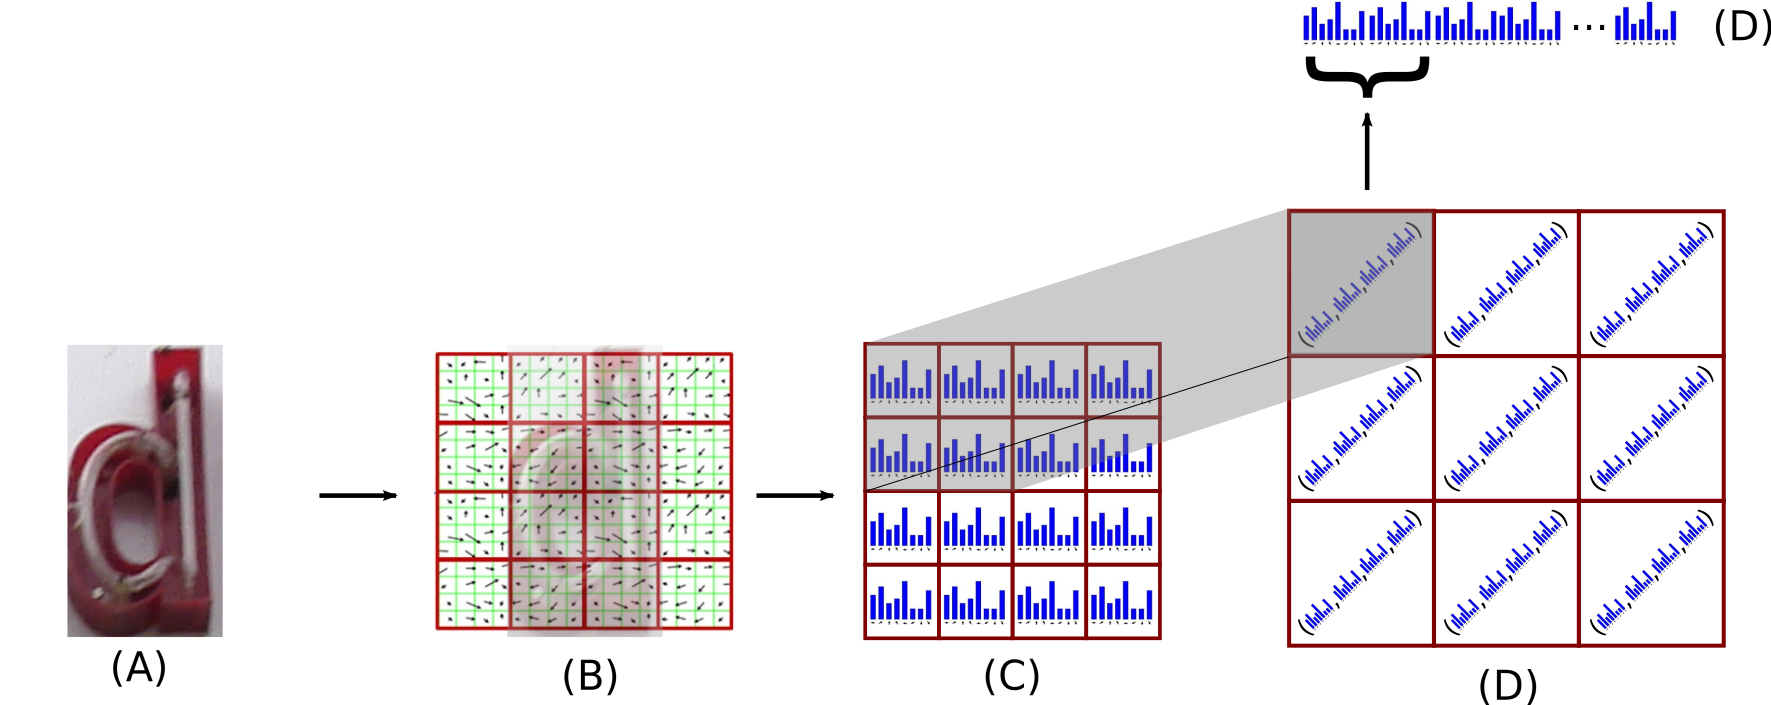
\includegraphics[scale=0.27]{img/hog/hog.png} }
			\caption[Extracción HOG]{Formación del vector de características HOG}
			\label{fig: Vector HOG}
		\end{figure}

	
	%\input{capitulo2/recon_objetos.tex}

	
	\subsection{Reconocimiento de caracteres}

	\begin{itemize}
		\item Algoritmos usados
			\begin{itemize}
				\item Introducción a Random Ferns: explicar el algoritmo y porqué lo usaron.
				\item HOG: hacer una ligera mensión de su uso. Los detalles van a estar en la sección correspondiente en el capítulo 2.
				\item non-maximal suppression (NMS)
			\end{itemize}
		\item Datasets usados
			\begin{itemize}
				\item Aca puede ir una explicación del uso de datos sintéticos.			
			\end{itemize}			 
	\end{itemize}
	
	\RC{Abajo, borrador}
	
	El reconocimiento de caracteres, es la primera etapa en el pipeline de procesamiento que desarrollaron Wang et al. Para esto, realizaron una detección a múltiple escala usando un algoritmo de clasificación de ventana deslizante. Dado que la cantidad de clases a detectar eran muchas (62 clases), ellos decidieron usar \textit{random ferns} como su clasificador. Esto es debido a que es un clasificador multi-clase y es eficiente.
	
	Random ferns fue explicado con anterioridad en la sección \ref{subsection:ferns}. Para la obtención de las características, los autores hacen uso de los descriptores HOG  los cuales binarizan (ver \ref{subsection:hog}) aplicando umbrales aleatorios con el objetivo de obtener vectores de características que puedan ser fácilmente almacenados y accesibles a través de una tabla. Como última etapa en el reconocimiento de caracteres, realizan \textit{non-maximal suppression} sobre cada carácter usando la siguiente heurística: iteran sobre todas las ventanas en la imagen en orden descendiente de su puntaje, si la ubicación no fue suprimida, suprimen todos sus vecinos.
	
	Uno de los problemas al entrenar un clasificador de caracteres, es el de encontrar un dataset de entrenamiento lo suficientemente grande para obtener buenos resultados. Una forma de solventar este problema, es generar un dataset con imágenes sintéticas, ya que, además de la  obvia ventaja de tener una cantidad ilimitada de datos, permite tener control sobre las dimensiones de cada imagen. Este enfoque fue aprovechado por Wang et al., que sintetizaron alrededor de 1000 imágenes por carácter usando 40 fuentes. A cada imagen, le agregaban una cierta cantidad de ruido gaussiano y le aplicaban transformaciones afines aleatorias. Con esto, obtenían imágenes de caracteres que intentaban asemejarse a las reales.
	
	
	
	%\subsection{Reconocimiento de palabras}
	\begin{itemize}
		\item Introducción a Pictorial Structures (Teoría)
		\item Uso de PS + Lexicón
		\begin{itemize}
			\item Algoritmo PLEX
		\end{itemize}
		\item Re-scoring y NMS
		\begin{itemize}
			\item Problemas con PLEX
		\end{itemize}
		\item Implementación
	\end{itemize}
	
	\subsection{Arquitectura del sistema}
\label{subsection:impl_propia}

	El presente trabajo, como se dijo con anterioridad, sienta sus bases en el trabajo realizado por Wang et al. salvo que el enfoque del mismo se centra en los problemas de reconocmiento de caracteres y el reconocimiento de palabras. En las próximas subsecciones, se procederá a explicar cuestiones de implementación que se tuvieron en cuenta al momento de resolver ambos problemas.

	\subsubsection{Reconocimiento de caracteres}
	\label{subsubsection:recon-caracteres}
		\paragraph{Pipeline de procesamiento} ~\\

			La implementación que se realizó en este trabajo, está basada en un pipeline similar al que realizaron Wang et al. que comprende dos instancias: la instancia de entrenamiento y la instancia de evaluación. La primera esta constituida por la generación de datos sintéticos que constituyen el conjunto de entrenamiento, la extracción de las características, la binarización y el entrenamiento del clasificador. La segunda instancia consiste en la evaluación del clasificador que abarca desde la extracción y binarización de las características del conjunto de prueba y posteriormente la evaluación del clasificador para cada una de estas. El pipeline se puede apreciar en la siguiente imagen:

			\begin{figure}[htbp]
				\centering
				\fbox{ \includegraphics[scale=0.5]{img/OCR_pipeline_1.jpg} }
				\caption[Pipeline de procesamiento]{Esto es un ejemplo de como quedaría visualmente pero no es el pipeline de este trabajo.}
				\label{fig: Pipeline de mi sistema}
			\end{figure}

		\paragraph{Generación de datos sintéticos} ~\\

			La datos sintéticos que se generan y utilizan en este trabajo son extraidos del dataset \textit{Chars74K} el cual está compuesto, entre otras cosas, por 62992 imágenes de caracteres sintéticos extraidos de fuentes de computadora. Cada una de las clases involucradas en la clasificación tienen un poco más de 1000 de estas imágenes (son 62 clases en total). El objetivo detrás de la generación de estos datos sintéticos es agregar vistas de los caracteres que no están reflejadas en el dataset original pero que son plausibles de ser observadas en la realidad.
			
			Inicialmente, se tiene como base un conjunto el cual contiene imágenes de caracteres de diversas fuentes. Lo que se busca, es aplicar a cada imagen un conjunto de transformaciones afines aleatorias con el objetivo final de obtener una imagen nueva con la apariencia  lo más cercana a una real. Una transformación afin representa en esencia una relación entre dos imágenes. La misma se aplica entre dos espacios afines (son estructuras geométricas que generalizan las propiedades afines del espacio Euclideo) y consiste en una transformación lineal seguida de una traslación. Formalmente, es una función entre espacio afines . Si $X$ e $Y$ son espacios afines, luego cada transformación afín $f:X \rightarrow Y$ es de la forma $x\mapsto Mx + b$, donde $M$ es una transformación lineal en $X$ y $b$ es un vector en $Y$. Se usan las multiplicaciones entre matrices para representar las transformaciones lineales y la suma de vectores para representar las traslaciones. Mediante matrices ampliadas, sin embargo, es posible representar ambos tipos de transformaciones.	La matriz $M$ presentada anteriormente es una matriz $2\times 2$ y permite realizar transformaciones en imágenes de 2 dimensiones. En este trabajo, para generar los datos sintéticos se hacen uso de las siguientes transformaciones:
			
			\paragraph{Rotación}
			
				La rotación es una transformación afín que consta en rotar el ángulo de la imágen en el sentido anti-horario. El parámetro usado para el mismo son los radianes y las diferentes variaciones se pueden apreciar en la figura \ref{fig: Transformacion Afin - Rotacion}. Teniendo en cuenta la definición formal de una transformación afín anterior, la rotación formalmente se puede representar de la siguiente manera:

			\begin{equation*}
					M =  
					\begin{bmatrix}
						cos(\theta) & -sin(\theta) \\
						sin(\theta) & cos(\theta)  \\
					\end{bmatrix}
					b =
					\begin{bmatrix}
						0 \\
						0 \\
					\end{bmatrix}	
			\end{equation*}

	donde se puede observar el parámetros $\theta$ que representa el grado de inclinación y el vector $b$ es nulo por lo cual no hay traslación alguna.

		\begin{figure}[htbp]
			\centering
			\subfloat[\label{fig: sintetica original}]{
				\fbox{ \includegraphics[scale=1]{img/transformaciones/original.png} }
			}
			\subfloat[\label{fig: Imagen rad 0.5}]{
				\fbox{ \includegraphics[scale=1]{img/transformaciones/rotation0,5.png} }
			}
			\subfloat[\label{fig: Imagen rad 1}]{
				\fbox{ \includegraphics[scale=1]{img/transformaciones/rotation1.png} }
			}
			\subfloat[\label{fig: Imagen rad 1.5}]{
				\fbox{ \includegraphics[scale=1]{img/transformaciones/rotation1,5.png} }
			}
			\caption[Rotación de un caracter]{Rotación de un caracter. (a) Imagen original. (b) Imagen rotada 0.5 radianes. (c) Imagen rotada 1 radian. (d) Imagen rotada 1.5 radianes}
			\label{fig: Transformacion Afin - Rotacion}
		\end{figure}	
			
		\paragraph{Escala}
			
			La escala es una transformación que busca modificar el tamaño del objeto al cual se la aplica haciendola más chica o más grande lo que era originalmente. Formalmente, se puede representar por la siguiente configuración de la matriz $M$:
			\begin{equation}
				M = 
				\begin{bmatrix}
					a & 0 \\
					0 & d \\
				\end{bmatrix}
			\end{equation}
		donde $a$ y $d$ representan los cambios en los ejes $x$ e $y$ de la imagen respectivamente. Se puede apreciar la aplicación de esta transformación en la figura \ref{fig: Transformacion Afin - Escala}.
		\begin{figure}[htbp]
			\centering
			\subfloat[\label{fig: escala original}]{
				\fbox{ \includegraphics[scale=1]{img/transformaciones/original.png} }
			}
			\subfloat[\label{fig: Imagen escala 0.8}]{
				\fbox{ \includegraphics[scale=1]{img/transformaciones/scale0,8.png} }
			}
			\subfloat[\label{fig: Imagen escala 1.2}]{
				\fbox{ \includegraphics[scale=1]{img/transformaciones/scale1,2.png} }
			}
			\caption[Cambio de escala de un caracter]{Cambio de escala de un caracter. (a) Imagen original. (b) Imagen ampliada $1.2$ veces su tamaño  (c) Imagen reducida a $0.8$ veces su tamaño .}
			\label{fig: Transformacion Afin - Escala}
		\end{figure}	
			
		\paragraph{Transvección}
		
			La transvección es una transformación donde la imagen se rota en un solo eje. Es una función que toma un punto con coordenadas $(x,y)$ al punto $(x +ny, y)$ donde $n$ es un parámetro fijo, denominado el factor de inclinación. El efecto es el desplazamiento de todos los puntos horizontalmente en una cantidad proporcional a su coordenada $y$. Todo punto encima del eje $x$ es desplazado a la derecha si $n > 0$, y a la izquiera si $n < 0$. Nuestra matriz $M$ va a ser de la forma:
			\begin{equation}
				M = 
				\begin{bmatrix}
					1 & n \\
					0 & 1 \\
				\end{bmatrix}.
			\end{equation}
		Se puede observar en la figura \ref{fig: Transformacion Afin - Transveccion} los diferentes efectos de aplicar diferentes valores de $n$ en la aplicación de la transvección en una imagen.
		\begin{figure}[htbp]
			\centering
			\subfloat[\label{fig: Imagen transveccion 0.5}]{
				\fbox{ \includegraphics[scale=1]{img/transformaciones/shear0,5.png} }
			}
			\subfloat[\label{fig: Imagen transveccion 0.2}]{
				\fbox{ \includegraphics[scale=1]{img/transformaciones/shear0,20.png} }
			}
			\subfloat[\label{fig: Imagen original}]{
				\fbox{ \includegraphics[scale=1]{img/transformaciones/original.png} }
			}
			\subfloat[\label{fig: Imagen transveccion -0.2}]{
				\fbox{ \includegraphics[scale=1]{img/transformaciones/shear-0,20.png} }
			}
			\subfloat[\label{fig: Imagen transveccion -0.5}]{
				\fbox{ \includegraphics[scale=1]{img/transformaciones/shear-0,5.png} }
			}
			\caption[Transvección de un caracter]{Cambio de transvección de un carácter.}
			\label{fig: Transformacion Afin - Transveccion}
		\end{figure}	
		
		\paragraph{Traslación}		
			
			La traslación es el último tipo de transformación afín que usamos en este trabajo y a diferencia del resto de las transformaciones, esta no hace uso de $M$, sino de $b$ que es el vector de desplazamiento. Formalmente:
			\begin{equation*}
				M =  
					\begin{bmatrix}
						1 & 0 \\
						0 & 1  \\
					\end{bmatrix}
					b =
					\begin{bmatrix}
						b_1 \\
						b_2 \\
					\end{bmatrix}	
			\end{equation*}
		donde $b_1$ y $b_2$ representan el movimiento en el eje $x$ e $y$ respectivamente. Particularmente no usamos esta transformación para mover los caracteres, sino más bien para mantener la imagen del carácter centrada durante las diferentes transformaciones que le aplicamos a la imagen.
		
		
		\paragraph{Suavizado Gaussiano}
		
			Es una técnica que consta de la difuminación de una imagen a partir de la aplicación de una función gaussiana. Se usa principalmente para reducir el ruido en una imagen. Dados das las coordenadas de un punto $(x, y)$ en una imagen, la función de suavizado es la siguiente
			\begin{align*}
				G(x,y) = \frac{1}{2\pi\sigma^2}\epsilon^{-\frac{x^2+y^2}{2\sigma^2}}
			\end{align*}
			donde $\sigma$ es la desviación estandard de la distribución gaussiana. En la figura \ref{fig: Suavizado Gaussiano}, se puede observar como distintos valores para $\sigma$ a medida que aumenta va distorcionando la imagen un poco más.
			
		\begin{figure}[htbp]
			\centering
			\subfloat[\label{fig: Imagen original sin blur	}]{
				\fbox{ \includegraphics[scale=1]{img/transformaciones/original.png} }
			}
			\subfloat[\label{fig: Imagen con blur 1}]{
				\fbox{ \includegraphics[scale=1]{img/transformaciones/blur1.png} }
			}
			\subfloat[\label{fig: Imagen con blur 2}]{
				\fbox{ \includegraphics[scale=1]{img/transformaciones/blur2.png} }
			}
			\caption[Suavizado Gaussiano de un caracter]{Aplicación de blur o suavizado gaussiano a un caracter. (a) Imagen original. (b) Imagen suavizada con un valor de $\sigma = 1$  (c) Imagen aún más suavizada con un valor de $\sigma = 2$ .}
			\label{fig: Suavizado Gaussiano}
		\end{figure}				
			
			
		\paragraph{Ruido Gaussiano}			
			
			El ruido en una imagen es una variación en la información sobre el color o la iluminación en la misma. Puede ser producido por un sensor, la circuitería de una escaner o una cámara digital. Condiciones de poca iluminación o interferencia electromagnética durante la transmisión de las imágenes son factores para que aparezca este tipo de distorsiones. El ruido gaussiano en las imágenes es un tipo de ruido que se caracteríza por tener una distribución gaussiana. La figura \ref{fig: Ruido Gaussiano} presenta 2 ejemplos de imágenes de caracteres con ruido gaussiano. A medida que el parámetro $\sigma$  aumenta, el ruido en la imagen se hace más notorio.
			
		\begin{figure}[htbp]
			\centering
			\subfloat[\label{fig: Imagen original sin ruido	}]{
				\fbox{ \includegraphics[scale=1]{img/transformaciones/original.png} }
			}
			\subfloat[\label{fig: Imagen con ruido 15}]{
				\fbox{ \includegraphics[scale=1]{img/transformaciones/noise15.png} }
			}
			\subfloat[\label{fig: Imagen con ruido 30}]{
				\fbox{ \includegraphics[scale=1]{img/transformaciones/noise30.png} }
			}
			\caption[Ruido Gaussiano en un caracter]{Aplicación de ruido gaussiano a un caracter. (a) Imagen original. (b) sigma=15  (c) sigma=30 .}
			\label{fig: Ruido Gaussiano}
		\end{figure}
			
			Un punto a destacar en este proceso, es que las fuentes de letras están en una escala de grises y se mantienen de esta forma. Esto es debido a que, durante el entrenamiento, solo es posible obtener las características de las imágenes sí y sólo sí estas están en escala de grises (requerimiento del algoritmo HOG). 
			
		\paragraph{Anexar caracteres}
					
			Otro tipo de modificación que vale la pena destacar, es la de anexar caracteres a los costados de la imagen a alterar. Esto es debido a que la mayoría de las imágenes de caracteres reales son extraidas de entornos donde la misma forma parte de una palabra. Es por eso que en la mayoría de los conjuntos generados, cada caracter está acompañado de pedazos de otros caracteres.
			
		\begin{figure}[htbp]
			\centering
			\subfloat[\label{fig: Imagen anexo 1	}]{
				\fbox{ \includegraphics[scale=1]{img/transformaciones/anexo1.png} }
			}
			\subfloat[\label{fig: Imagen anexo 2}]{
				\fbox{ \includegraphics[scale=1]{img/transformaciones/anexo2.png} }
			}
			\subfloat[\label{fig: Imagen anexo 3}]{
				\fbox{ \includegraphics[scale=1]{img/transformaciones/anexo3.png} }
			}
			\caption[Caracteres pegados]{Imágenes de caracteres con caracteres pegados a izquierda y derecha.}
			\label{fig: Imagen anexos}
		\end{figure}

			La creación de estos datos sintéticos son para el conjunto de entrenamiento del clasificador. El conjunto de test esta conformado por 15 imágenes reales por clase obtenidas del dataset \textit{Chars74K-15}, a las cuales no se les modifico en absoluto. Esto es debido a que los experimentos de evaluación del clasificador que se realizen tienen que poder ser comparados con los de Wang et al. en iguales condiciones.


		\paragraph{Entrenamiento del clasificador}  ~\\

			La segunda etapa del pipeline corresponde al entrenamiento del clasificador. Al igual que los autores del trabajo original, en este se utiliza como clasificador a Random Ferns. Para poder entrenar al clasificador, se procede a extraer las características de las imágenes del conjunto de entrenamiento a través del algoritmo HOG. HOG devuelve en sí un vector $v \in \mathbb{R}^{n}$ (donde $n$ depende de los parámetros que se le pasen al algoritmo, explicado en el próximo capítulo) el cual hay que binarizar para poder almacenarlo.

			Para poder binarizar los vectores calculados, como se explicó en la sección \ref{subsection:hog}, se necesita de un umbral cuya dimensión es igual a la de los vectores. Dicho umbral binariza a un vector comparando sus valores dimensión a dimensión. Un vez realizado este procedimiento, los vectores modificados se almacenan en un diccionario. Este último, esta estructurado como un conjunto de diccionarios anidados y representa la base ``base de datos'' del sistema. Los detalles del porqué se eligió esta forma de almacenar la información se puede encontrar en el apéndice A. \RC{Crear apendice A donde se van a discutir cosas como lenguaje usado, base de datos, librerias entre otros}

			Dado que los vectores pertenecen al conjunto $\{ 0,1 \}^{N}$ si los quisiéramos almacenar en una sola tabla (habría una tabla por clase), cada una debería tener $2^{N}$ entradas lo cual si $N$ es muy grande sería imposible por la cantidad de memoria necesitada para mantener estas tablas en memoria. Luego, basándonos en lo explicado sobre Random Fern en \cite{subsection:ferns}, la solución pasa por dividir cada vector en $M$ grupos de dimensión $S = \frac{N}{M}$. Con esto, un vector completo esta almacenado en $M$ tablas diferentes (tablas correspondiente a la clase del vector). En total estaríamos trabajando con $M \times 62$ tablas (pues hay 62 clases diferentes).

			Dado un vector $v=(v_1, \dots, v_s)$ donde $v_i \in \{ 0,1 \}^{M}$, $z$ sea la clase de $v$ y sean $t_i i=1, \dots, s$ las tablas de $z$. Cada grupo $v_i i=1, \dots, s$ va a tener una entrada en su tabla correspondiente $z_i$ equivalente a su representación decimal. Inicialmente cada tabla está inicializada dado un parámetro $\alpha \neq 0$ que se explicará en detalle en el próximo capítulo.

		\paragraph{Evaluación del clasificador} ~\\

			Para la evaluación del clasificador, se toma como conjunto de test el descripto en la sección de descripción del dataset. A cada imágen del conjunto de test, se le extrae el descriptor HOG, se lo binariza y con el vector resultante se calcula la probabilidad de que dicho vector perteneza a cada una de las clases involucradas. El calculo para cada clase es el mismo y consiste en dividir el vector de prueba en $M$ grupos y por cada grupo obtener el valor en la tabla correspondiente. Por cada clase entonces tendríamos $M$ valores. Finalmente se realiza la suma de los logaritmos de cada valor y el resultado es la probabilidad de que ese vector pertenzca a la clase evaluada. Como es claro, al final se le asigna a la imagen evaluada la clase que haya obtenido la mayor probabilidad.

	\subsubsection{Reconocimiento de palabras}

		\RC{Todavía no he implementado nada de esto así que queda pendiente...}

